% !Mode:: "TeX:UTF-8"

\chapter{引言}
\label{ch:intro}

根据天津大学模板修改的符合中山大学毕业论文(至少是硕士论文)要求的Latex模板。

\section{使用方法}
\label{sec:usage}

本模板只包括内容方面的设计预定义,编译自行解决。作者使用的是Windows环境下MikTex+TeXstudio的组合。

\section{使用建议}
\label{sec:tips}

\subsection{普适问题}
\label{subsec:common}

普遍适用的论文排版问题:

\begin{itemize}
\item 图片标题在下,表格在上;一定要有标题,不能只是图1-1;与文字内容的间隔自行把握。
\item 参考文献建议使用.bib文件;也有使用Google Scholar的引用的,但有指出当中的“//”不符合规范。
\item 部分评审反馈,目录不包含摘要及目录本身,请根据情况自行斟酌。
\item 打印时需要右边翻页的问题(每章开始在右边页),可以在生成pdf后通过插入空白页解决(这样插入不会改变页码);或者尝试设置openright(未测试,有待探讨)。
\end{itemize}

\subsection{细节问题}
\label{subsec:specs}

一些细节的问题建议:
\begin{itemize}
\item 每个章节都有label,key使用ch:intro形式,以下使用sec:background等。图片key可以参考fig:scenes,表格参考tab:exp。
\item 图片、表格尽量在页的顶部,即float优先选择t。
\item 另外,为了打印时彩打方便,可以把需要彩打的图片尽量排版在一页,不过比较难调。
\item 虽然每个body的tex文件中包含了!Mode:: ``TeX:UTF-8"在文件开头,但仍有必要在IDE中将新建的tex文件设为UTF-8编码,否则可能无法正常显示中文。
\end{itemize}

\subsection{其他说明}
\label{sec:setting}

参考文献\cite{wu2013online}目前采用上标表示。使用cite命令。

目前页眉设置:每章第一页页眉只有中间的“中山大学硕士毕业论文”,后续页左边显示“中山大学硕士毕业论文”,右边显示“第n章”。

目前页脚设置:仅包含页码,居中,无横线。

参考文献和附录计算页数,包含在目录,页眉设置同每章第一页。正文前的部分无页眉。

\section{例子}
\label{sec:examples}

图例子。label要在caption后。多图或子图方法上网查吧。

\begin{figure}[!t]
	\centering
	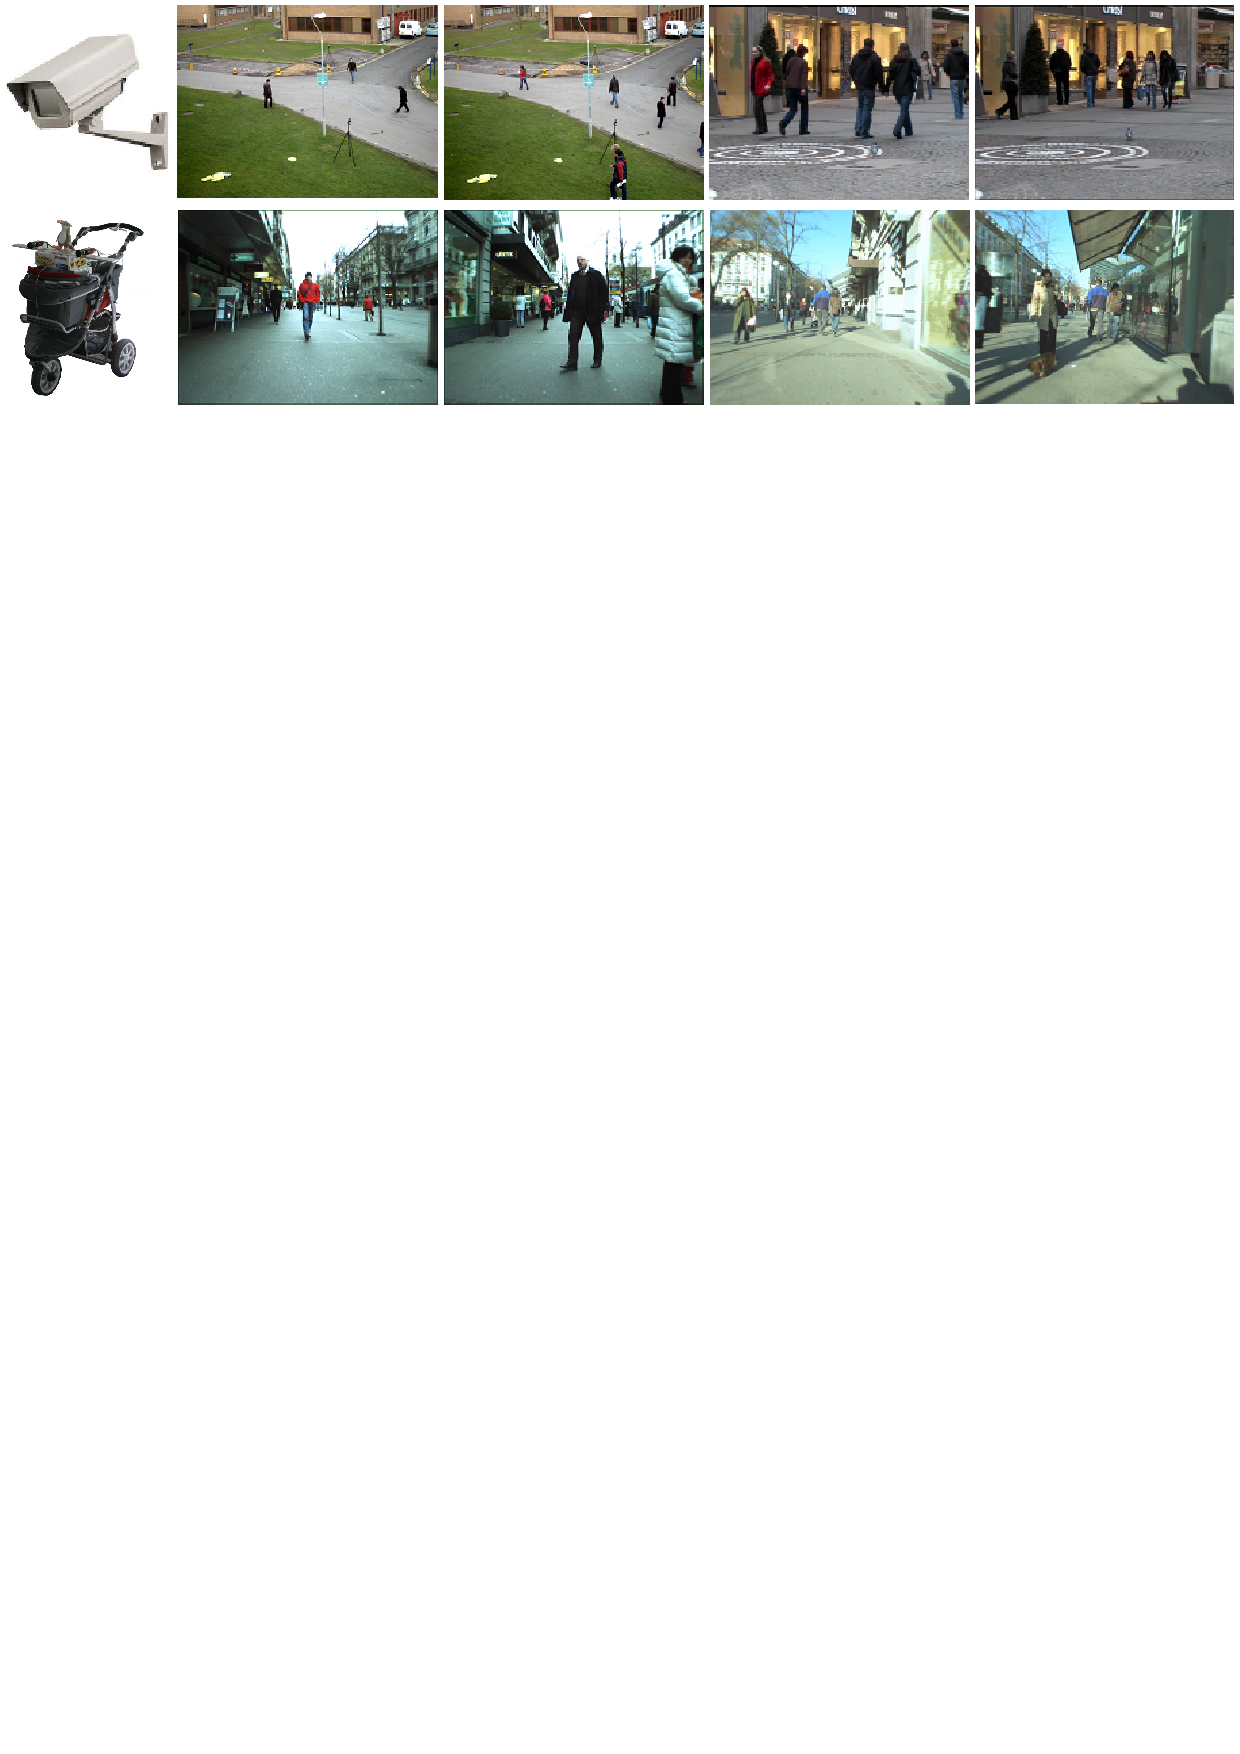
\includegraphics[width=0.95\textwidth]{scenes}
	\caption{图例}
	\label{fig:scenes}
\end{figure}

表例子。推荐使用这种三行表。缺省值使用三个“-”产生长横线“---”。

\begin{table}[!t]
\caption{示例表}
\label{tab:eg}
\vspace{0.5em}
\centering
\wuhao
	\begin{tabular}{ccccc}
	\toprule[1.5pt]
	表头 & 栏1 & 栏2 & 栏3 & 栏4 \\
	\midrule[1pt]
	内容1 & b & --- & $768 \times 576$ & 19 \\
	内容1 & a & 240/7 & $768 \times 576$ & --- \\
	\bottomrule[1.5pt]
	\end{tabular}
\end{table}

公式例子,与普通Latex数学公式无异。

\begin{equation}
1+1=2
\end{equation}

\section{章节安排}

